\documentclass[tikz]{standalone}

\definecolor{coral}{rgb}{1.0, 0.5, 0.31}    % Defining coral
\definecolor{maroon}{rgb}{0.5, 0.0, 0.0}    % Defining maroon
\definecolor{plum}{rgb}{0.933, 0.196, 0.2}   % red
\begin{document}
	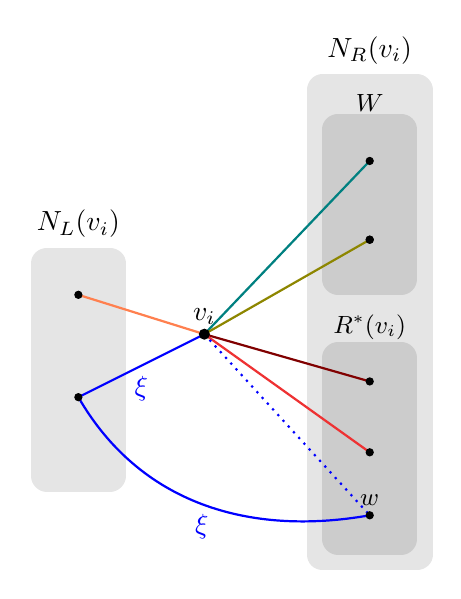
\begin{tikzpicture}
		\filldraw [line width=4mm,join=round,black!10]
		(0,1) rectangle (0.8,3.7) 
		(3.5,0) rectangle (4.7,5.9);
		
		\filldraw [line width=4mm,join=round,black!20]
		(3.7,0.2) rectangle (4.5,2.5)
		(3.7,3.5) rectangle (4.5,5.4);
		
		\coordinate (v) at (2,2.8);
		
		\node[above,font=\small] at (4.1,2.6) {$ R^*(v_i) $};
		\node[above,font=\small] at (4.1,5.5) {$ W $};
		\node[above,font=\small] (uu) at (4.1,0.5) {$ w $};
		
		\node[above] at (2,2.8) {$ v_i $};
		\node[above] at (0.4,3.9) {$ N_L(v_i) $};
		\node[above] at (4.1,6.1) {$ N_R(v_i) $};
		
  		\draw[thick, coral] (v) -- (0.4,3.3);    % Coral line
		\draw[thick, teal] (v) -- (4.1,5);       % Teal line (teal is a predefined color)
		\draw[thick, olive] (v) -- (4.1,4);      % Olive line (olive is a predefined color)
		\draw[thick, maroon] (v) -- (4.1,2.2);   % Maroon line
		\draw[thick, plum] (v) -- (4.1,1.3);     % Plum line
		
		\draw[thick,color=blue] (v) -- (0.4,2) node[midway,color=blue,below]{$ \xi $};
		\draw[thick,color=blue,dotted] (v) -- (4.1,0.5);
		
		\draw[thick,color=blue,out=-60,in=-170] (0.4,2) edge node[color=blue,below]{$ \xi $} (4.1,0.5);
		
		\fill (v) circle (2pt);
		\fill (0.4,3.3) circle (1.5pt);
		\fill (4.1,5) circle (1.5pt);
		\fill (4.1,4) circle (1.5pt);
		\fill (4.1,4) circle (1.5pt);
		\fill (4.1,2.2) circle (1.5pt);
		\fill (4.1,1.3) circle (1.5pt);
		\fill (0.4,2) circle (1.5pt);
		\fill (4.1,0.5) circle (1.5pt);
	
	\end{tikzpicture}
\end{document}
